%===================================== CHAP 5 =================================

\chapter{Approach}

Utsida is a joint collaboration between two students with specializations in software- and an artificial intelligence, respectively. This is reflected by a two-part system were each part targets one of the research questions. This chapter will define how the complete system is build, how the CBR part is modelled, elaborate for choices made, and how it works.

Utsida was chosen as the name of the system due to being a counter opposite to NTNU's central system \emph{Innsida}, and the meaning of the word \emph{inside}. Utsida gives a relation to something on the outside, in this case going on an exchange study, choosing a foreign university, and a set of courses at that university. Utsida is a web application, and serves as the platform which the users use. This chapter covers the overlying architecture, the web part, CBR REST, the development process, about the design, and the data used in the system.

\section{Knowledge acquisition}

The system required an extensive amount of external data to be relevant. Data from several sources was acquired and is listed below.

\begin{itemize}
    \item Experience Reports: The data source used to construct cases for the case-base. Explained in section \ref{sec:experience_reports}. Also used for a heatmap of popular exchange countries. 
    \item Assessed course matches at NTNU: Logged by some advisers at NTNU in different format. Was manually parsed to create an initial base of assessed course matches in Utsida.
    \item Courses at NTNU: Filled in Utsida's database from IDI's organizational API for NTNU. 
    \item Faculties and institutes at NTNU: Also filled in Utsida's database from IDI's organizational API for NTNU.
\end{itemize}

\subsection{The Experience Reports}\label{sec:experience_reports}
Typically, a CBRS' case-base is gradually filled as a new case arrives. In this project, it was essential to have a large number of cases in the case-base from the start. A large part of the motivation for doing this research stems from personal experience, and thus it the current process at NTNU was well known. Most students who go on an exchange program at NTNU has to write obligatory reports to NTNU's International Section. These reports are public, and because of all the information about an exchange study they included, they proved to work as a great base for a case. All of the current public experience reports were downloaded, and parsed (see section \ref{sec:parser}) to cases, and filled in the CBRS' case-base. With this in place, the data and foundation of the CBRS was in place.

\subsection{Parsing the Experience Reports}

\subsection{Data Quality}
Cleaning and validating the data was a large part of the preparation process. The data detailed in the previous chapter was not uniform and allowed in many cases free text entry. This caused the data to have large differences in both structure and entries. The data was analyzed according to the six primary dimensions for data quality assessment\cite{askham2013six} as further detailed in the following paragraphs.

\paragraph{Completeness}
Many of the experience reports which were parsed was not complete at all. This was an issue if the missing data included the student's institute, or which subjects they chose. This was completely necessary data because the institute was the biggest factor which made a case relevant for a user of Utsida, while the subjects is the solution to each case; without them the case doesn't help much. Therefore, any reports which was missing this data was automatically excluded by the parser.

\paragraph{Uniqueness}
There seems to be a good uniqueness in the cases in the way that there are visible repetition of exchange experiences from the same person. Since the underlying exchange experiences are anonymous there was no way to check for number of individual persons submitted a experience versus the number of experiences in total. 

\paragraph{Timeliness} 
is the "The degree to which data represent reality from the required point in time"\cite{askham2013six}. The last submitted experiences in the data set is from 2015 and the first ones from 1999. The data set should include entries from 2017 but the experience submission system was put on hold from 2015 and changed in early 2017. This means the newest data is already 2 years old at the time of this writing. The experiences tend to be submitted either a couple of months after an exchange period or in the middle of one. This makes the timeliness have a great degree of variation and is difficult to assess. 


\paragraph{Validity} Most of the data was not validated in any way. There were lack of data input requirements, data type constraints, range constraints and membership constraints. This was especially the case for the exchange experiences and the approved course replacements.


\paragraph{Accuracy}
The data used to parse into cases for the CBRS was mostly raw text. Obviously, attributes came in all forms of abbreviations and ways to write the same thing. Utsida on the other hand required strict uniform formats on every input. A partly solution to this issue was solved by creating data dictionaries with all possible attributes on the format which was required by Utsida. The input was then matches to each of these entries in the dictionary with Approximate string matching, or Fuzzy Searching. This approach returns the most similar entry in the pre-defined dictionary to the input attribute, and ensured the data holds the same format. 

Not all problems regarding accuracy was possible to avoid however. Because input attribute for which university a student went to, and which subject they took is a subset of a such enormous set of data, that it is not possible to keep all alternatives in a pre-defined format. Atleast not with any APIs available today.


\paragraph{Consistency}
Most of the reports are written in Norwegian, which means there are many characters which has to be encoded and decoded between UTF-8 and Ascii text standards. The parser was initially generating a JSON object of all the parses cases, but its encoding crashed with that in MyCBR. To avoid this, the JSON step was skipped, and the data was parsed directly from the experience report to a case in CSV format.

\subsection{Fuzzy Searching on Data}
As mentioned, the cases used in Utsida's CBRS are essentially simplified data representations of the experience reports. These reports contain many fields where the student who writes it can write the answers with free text, rather then selecting from a predefined selection of alternatives. This proved to be an issue when parsing the data into cases, because a more strict format on each attribute was required. The script parsing each experience report therefore had to take care of a lot of edge-cases, and reformat the student's answers into our own format. A method proved to be extremely useful in this situation, namely \emph{Fuzzy Searching}

Fuzzy Searching, or Approximate string matching, is an algorithm used to recognize patters and similarities in text, and yield a score to determine the similarity between them. Using technique in the script which parsed the experience reports, predefined sets of attributes could be formatted as the system required, and use fuzzy search on the text input in the reports, to map the most similar occurrences to our predefined data. For example, in the field in the reports where the student's wrote their institute at home, a huge variation of abbreviations, and other ways to write it is an issue. By creating a dictionary with all institutes and faculties, fuzzy searching could be used to match the input in the report to this dictionary, and return the record in the dictionary with the highest similarity score to the input in the report. This method was also used to avoid creating multiple instances of the same university in the database, because they were written slightly different.

\section{Architecture}

Some default functions in Django was extended to provide required functionality in the Utsida system. The user object was extended with profile information so that the system could register more information about the user such as institute and courses to be taken. 

The picture below is a rough draft of how the system architecture is and the communication with MyCBR. Utsida is divided into four main components; The recommendation handler communicates with the REST myCBR API and display the results for a given query. The Course Match component contains and displays all approved and registered course matches between NTNU and exchange universities. The profile handles all user controllers, such as login, logout, register and changing information. The course application allows users to register an application for course matches so that it can be handled by an student adviser. 

\begin{figure}[H]
    \centering
    \includegraphics[width=8cm]{fig/systemRepresentationDraft.png}
    \caption{Utsida Architecture}
    \label{fig:utsida}
\end{figure}

Typically in a CBRS, the results would be the solution of the case from the case-base with the highest similarity to the proposed problem, applied to this problem. Utsida does not recieve one solution, and does not apply any solution by itself to the user's query, but it lists the cases with the most similarity to the user's query. Therefore, Utsida is not a standard CBRS, but rather a Case Based Recommender System. This way, the user can browse several solutions, and pick the one they want.

\subsection{Django}
Django\cite{djangodocs} is a web framework using the Python programming language, and is maintained by the \enquote{Django Software Foundation} (DSF). The DSF calls it an \emph{MTV} framework, meaning \emph{Model, Template, View}, which in practice functions as a \emph{MVC} pattern. It comes bundled with a lightweight database, a predefined directory structure, controllers to handle any communication between the different components, and many other package. Most noteworthy: Django's security packages, which handles important security risks such as Cross-Site Request Forgery and authorization, and the administrator panel, which lets the developers easily manage entries in the database with an intuitive interface. Everything Django offers completes a package which essentially lets developers focus on their ideas and the application, instead of structural difficulties. 

As the title suggests, Django is a good choice for projects with slim time schedules, and rapid change, which ultimately is the reason for this choice of framework.

\section{RESTful CBR}
Since the MyCBR SDK requires a Java environment, an initial problem was how to couple this functionality with a web application, which Utsida is. Luckily, Kerstin Bach, researcher at the Department of Computer and Information Science, NTNU is a contributor to the MyCBR project, and implemented the basis for a REST (Representational State Transfer) framework for a running MyCBR application. The CBR part of the system could then be a separate module, communicating with Utsida only with HTTP requests.


\subsection{Case Representation in Utsida}

When parsing the experience reports, choices had to be made in regards to what data was needed. One of the most important aspects of Utsida, is that it should be fast and simple to use. Therefore, the amount of attributes and data extracted from the reports were initially narrowed down to a minimum, but still chose the data which yielded the most importance. The initial chosen data and attributes were modelled to the key-value pairs in table \ref{tab:case_representation1}.


\begin{table}[h]
\centering
\small
\caption{Initial representation of a case in Utsida}
\label{tab:case_representation1}
\begin{tabulary}{\textwidth}{|L|L|}
\hline
\rowcolor[HTML]{C0C0C0} 
\textbf{Attributes} & \textbf{Example Case} \\ \hline
\textbf{Home Institute} & IME-IDI - Institutt for datateknikk og informasjonsvitenskap \\ \hline
\textbf{Destination Continent} & North America \\ \hline
\textbf{Destination Country} & USA \\ \hline
\textbf{Destination University} & UCLA \\ \hline
\textbf{Study Language} & English \\ \hline
\textbf{Study Period} & 2012 \\ \hline
\textbf{Academic Quality Rating} & 4 \\ \hline
\textbf{Social Quality Rating} & 2 \\ \hline
\rowcolor[HTML]{8AD5EA} 
\textbf{Subjects Taken} & \begin{tabular}[c]{@{}l@{}}COMP1927 - Computing 2\\ MATH3220\\ CS4210\\ DATA101\end{tabular} \\ \hline
\end{tabulary}
\end{table}


This representation was used during the first usability testing of the system, which included an interview. From this, new information about good attributes to include was acquired, such as ease of finding a place to live, the standard of said place, the amount of support the students received at their chosen university, and the general cost of living in the country. These results lead to a an extended case representation, which is displayed in table \ref{tab:case_representation2}. This revision also spliced several ratings which was significant for the social aspects into the social quality rating, and the same for the academic.

\begin{table}[h]
\centering
\small
\caption{Extended representation of a case in Utsida}
\label{tab:case_representation2}
\begin{tabulary}{\textwidth}{|L|L|}
\hline
\rowcolor[HTML]{C0C0C0} 
\textbf{Attributes} & \textbf{Example Case} \\ \hline
\textbf{Home Institute} & IME-IDI - Institutt for datateknikk og informasjonsvitenskap \\ \hline
\textbf{Destination Continent} & North America \\ \hline
\textbf{Destination Country} & USA \\ \hline
\textbf{Destination University} & UCLA \\ \hline
\textbf{Study Language} & English \\ \hline
\textbf{Study Period} & 2012 \\ \hline
\textbf{Academic Quality Rating} & 8 \\ \hline
\textbf{Social Quality Rating} & 4 \\ \hline
\textbf{Ease to find- and quality of residential} & 5 \\ \hline
\textbf{Support and reception at university} & 6 \\ \hline
\rowcolor[HTML]{8AD5EA} 
\textbf{Subjects Taken} & \begin{tabular}[c]{@{}l@{}}COMP1927 - Computing 2\\ MATH3220\\ CS4210\\ DATA101\end{tabular} \\ \hline
\end{tabulary}
\end{table}

To finalize the case model, and also to form a basis for how important each of these attributes should be in a query, a questionnaire was sent out to a selected group of students (see chapter \ref{chap:3}).

\subsubsection{The Problem Part}

The following list elaborates the choice and significance of the different attributes used in a case.

\begin{itemize}
\item \textbf{Home Institute:} The home institute is considered the most important attribute, as it contains information about the student's faculty and institute at home, as well as a pointer to what kind of subject are relevant to the student. This also uncovered during the initial usability testing of the system; even though the geographical location and university, as well as every other factor seemed like a perfect fit, the suggestion is not valid if the suggested courses are irrelevant for the user. 

\item \textbf{Destination Continent:} The continent is included both give the user the opportunity to filter countries based on a continent, and to be able to only choose a continent if they are unsure of which country they would like to go to. 

\item \textbf{Destination Country:} The country serves as the most specific geographical option.

\item \textbf{Destination University:} The university is included to match exact universities in a case, if the user knows exactly which university they would go to.

\item \textbf{Study Language:} The study language represents they language which was reportedly used in a case.

\item \textbf{Study Period:} The study period is included to make older cases less relevant to the user, as a university's infrastrucre often changes over time. The option is hidden, and thus not selectable to the user. 

\item \textbf{Academic Quality Rating:} A rating which is a collaboration of an experience report's \emph{Academic Quality}, \emph{Special Competence Gained} and general \emph{Quality of Academic Opportunities}.

\item \textbf{Social Quality Rating:} A rating which is a collaboration of an experience report's rating of  \emph{Social Quality}, \emph{Leisure Activities}, \emph{Girlfriend/friends}, the social interaction with \emph{Students from the University}, \emph{Other Foregin Students} and \emph{Norwegian Students}.

\item \textbf{Ease to find- and Quality of Residential:} A rating which is a collaboration of an experience report's rating of \emph{Residential Dissemination} and \emph{Residential Quality}.

\item \textbf{Support and Reception at University:} A rating which is a collaboration of an experience report's rating of \emph{General Reception} and \emph{Administrative Support}.
\end{itemize}

It is important to note that a query in Utsida is doable with any number of selected attributes, the more attributes which are selected, the more relevant the results will be. 


\subsubsection{The Solution Part}
The solution to each case is the subjects the student chose. Considering another struggle for students wanting to do a study exchange is to chose an university as well, the chosen university can also be viewed as a solution to the case. With the mentioned attributes in place, the solution (the chosen subjects) should be relevant for the student, while the location should be feasible. 

\subsection{Taxonomies}
According to Michael M. Richter & Rosina O. Weber\cite{richter2013case}, taxonomies are widely used structures and specialisations of graphs. They relate
objects to each other. The intention is to do this in a hierarchical way, going from
general to more specific objects. This implies that branching leads to objects that
have more in common. 

In Utsida's CBR model, several attributes are a perfect fit for using a taxonomy to organize objects directly. For example, if a query contains a country, instead of only yielding a similarity score on how good this country matches with the country in each case, it will also yield a given similarity score if the country resided within the same continent as the country in the query. Figure \ref{fig:country_taxonomy} illustrates how the taxonomy for a country's similarity score is modelled in Utsida.

\begin{figure}[H]
    \centering
    \includegraphics[width=0.8\textwidth]{fig/country_taxonomy.png}
    \caption{Brief illustration of the taxonomy for the country attribute}
    \label{fig:country_taxonomy}
\end{figure}

If the country in a query is an exact match with the country in a case, the similarity score for the country attribute in that case will be 1.0. If it is a different country, but it still resides within the same continent as the country in a case, it will yield a similarity score of 0.3. No match at all will yield a 0.0. The same taxonomy is in place for the \emph{Home Institute} attribute, albeit ordered under the different faculties instead. Thus the faculty also works as a hidden attribute.

\subsection{Attribute Similarity Measures}

\begin{itemize}
    \item \textbf{Rating Similarity:} In the case-model, the attributes \emph{AcademicQuality}, \emph{SocialQuality}, \emph{ReceptionQuality} and \emph{ResidentialQuality} are conjunctions of different ratings given in the experience reports. Each rating ranges between 1-10, and reflects how the student experienced their trip with regard to these categories. To calculate the similarity between a rating in a case, and a rating from a query, the CBRS uses Symmetric Difference Determined Similarity\cite{bergmann2002experience} with a linear function. It describes the decrease in similarity depending on the increase of the difference at a linear phase.
    
$\begin{displaystyle}
    f(d) = 
    \begin{cases} 1 : & d < min \\ 
    \frac{max-d}{max-min} : & min \leq d \leq max \\
    0 : & d > max
    \end{cases}
\end{displaystyle}$

    \item \textbf{Continent Similarity:} The continent attribute is a \emph{Symbol type}, meaning its allowed values are a pre-determined set. Similarity between continents are calculated with a $m x n$ matrix, where each mapping yields a given similarity, as displayed in table \ref{tab:continent_similarity}. The values are rough estimates with regards to similarity in culture, language, location and general university structure.

    \begin{table}[H]
    \small
    \centering
    \caption{The $m x n$ matrix for calculating similarity between continents}
    \label{tab:continent_similarity}
    \begin{tabular}{|
    >{\columncolor[HTML]{C0C0C0}}l |
    >{\columncolor[HTML]{FFFFFF}}r |
    >{\columncolor[HTML]{FFFFFF}}r |
    >{\columncolor[HTML]{FFFFFF}}r |
    >{\columncolor[HTML]{FFFFFF}}r |
    >{\columncolor[HTML]{FFFFFF}}r |
    >{\columncolor[HTML]{FFFFFF}}r |}
    \hline
    Attribute value & \cellcolor[HTML]{C0C0C0}South America & \cellcolor[HTML]{C0C0C0}Asia & \cellcolor[HTML]{C0C0C0}Europe & \cellcolor[HTML]{C0C0C0}Africa & \cellcolor[HTML]{C0C0C0}North America & \cellcolor[HTML]{C0C0C0}Oceania \\ \hline
    South America & 1.0 & 0.0 & 0.2 & 0.0 & 0.3 & 0.0 \\ \hline
    Asia & 0.0 & 1.0 & 0.0 & 0.0 & 0.0 & 0.0 \\ \hline
    Europe & 0.2 & 0.0 & 1.0 & 0.0 & 0.2 & 0.2 \\ \hline
    Africa & 0.0 & 0.0 & 0.0 & 1.0 & 0.0 & 0.0 \\ \hline
    North America & 0.3 & 0.0 & 0.2 & 0.0 & 1.0 & 0.2 \\ \hline
    Oceania & 0.0 & 0.0.0 & 0.2 & 0.0 & 0.2 & 1.0 \\ \hline
    \end{tabular}
    \end{table}
    
    \item \textbf{Language Similarity:} In the experience reports, the language field promoted a free-text answer. To handle this, the experience report parser created a list of all languages mentioned in this answer, and added it to the case. Thus, the Language attribute in a case is a list of strings. The attribute is represented as a \emph{Symbol} type which allows multiple values, such as a list. The function used to calculate the similarity between a query attribute and a case attribute simply yields a similarity of $1.0$ if it is an exact match (for example if a query contains the Language attribute \emph{Spanish}, and a case has the same in its Language field). If such a query was matched with a case with the list of the languages \emph{English, Spanish}, it returns the mean similarity for each item in the list. In this case, it would return a similarity of $0.5$, because it simply yields a $1.0$ for \emph{Spanish} and $0.0$ for \emph{English}.
\end{itemize}

\subsection{Sum Functions}
Before giving each case in the case-base a similarity score based on a query, the result of the similarity measure on each attribute is summarized, with regards to the attribute's weight. These functions are called Multi-Criteria Decision Making Methods (MCDMM).

Among the available sum functions in the MyCBR Workbench, there are two widely used and suitable functions to use, namely the Weighted Sum Model (WSM) and the Euclidean Distance (ED). For single dimensional problems (such as in this system), the WSM can be used without difficulties, and is probably the most common approach \cite{triantaphyllou2000multi}, and is given by the following expression \cite{fishburn1967letter}

\begin{displaymath}
    A^{*}_{WSM-score}\quad =\quad max_{i}\  \sum\limits_{j = 1}^{n}\  a_{ij}w_{j},\quad for \quad i =1,\ 2,\ 3,\ ...,\ m.
\end{displaymath}

When the CBRS receives a query from Utsida, a decision matrix is calculated for each case. This is a $(m \times n)$ matrix whre each row is the attribute values of a case, paired with that attributes weight. 


\begin{table}[h]
\centering
\caption{A typical decision matrix for a query from Utsida to the CBRS}
\label{tab:decision_matrix}
\begin{tabular}{lllcccl}
                      &                       &                       & \multicolumn{1}{l}{} & \multicolumn{1}{l}{} & \multicolumn{1}{l}{} &                       \\
Attribute             & $Country$             & $Language$            & \ldots               & \ldots               & \ldots               & $AcademicQuality$     \\\hline
Weight                & $w_{country}$         & $w_{language}$        & \ldots               & \ldots               & \ldots               & $w_{country}$         \\\hline
$case_{1}$            & $sim_{case_{1}}$      & $sim_{case_{1}}$      & \ldots               & \ldots               & \ldots               & $sim_{case_{1}}$      \\
$case_{2}$            & $sim_{case_{2}}$      & $sim_{case_{2}}$      & \ldots               & \ldots               & \ldots               & $sim_{case_{2}}$      \\
\multicolumn{1}{c}{.} & \multicolumn{1}{c}{.} & \multicolumn{1}{c}{.} & \ldots               & \ldots               & \ldots               & \multicolumn{1}{c}{.} \\
\multicolumn{1}{c}{.} & \multicolumn{1}{c}{.} & \multicolumn{1}{c}{.} & \ldots               & \ldots               & \ldots               & \multicolumn{1}{c}{.} \\
\multicolumn{1}{c}{.} & \multicolumn{1}{c}{.} & \multicolumn{1}{c}{.} & \ldots               & \ldots               & \ldots               & \multicolumn{1}{c}{.} \\
$case_{m}$            & $sim_{case_{m}}$      & $sim_{case_{m}}$      & \ldots               & \ldots               & \ldots               & $sim_{case_{m}}$     
\end{tabular}
\end{table}

The WSM is used on this matrix to finally give each case in the case-base a similarity score between $0-1.0$, with regards to the query which the CBRS received. The CBRS then returns the list of the most relevant cases back to Utsida, which handles the rest.


\subsection{Weighting the Attributes}

Each attribute in a case has a value, and an associated weight. This is essentially just an integer denoting the importance of that attribute. During the modelling of the MyCBR project, these weights were chosen by the authors based on personal experience. These weights were in place during the usability testing, to learn if they seemed appropriate or not. To get a more public agreed upon set of weights, a questionnaire was sent out to a set of relevant student where they were asked to give their opinion of what kind of attributes were the most important when selecting location and courses for an exchange study, and specifically how important each of these attributes were. 

The questionnaire had 84 participants, where 36 answers included textual answers describing important factors for choosing a location for their exchange study. All of the answers included a numerical rating between 1-7, describing how important they think each of the attribute in the questionnaire was, where these attributes represents the attributes in a case-model. The numerical data was analyzed in a statistical manner, where the mean, standard deviation and coefficient of variation was calculated for each attribute. These statistical approaches was possible to use because most of the data turned out to be relatively normally distributed. Table \ref{tab:attribute_ranking} shows the values for each attribute scaled to a range between 1-10, while appendix \ref{appendix:word_frequency} displays the most frequent category of words in the textual answers.

\begin{table}[H]
\small
\caption{Statistical results from the questionnaire. \\ *SD: Standard Deviation, CV: Coefficient of Variation}
\centering
\label{tab:attribute_ranking}
\begin{tabulary}{\textwidth}{LRRR}
\textbf{Attribute} & \textbf{Mean (1-10)} & \textbf{SD (1-10)} & \textbf{CV (0-1)} \\ \hline
Study language & 8.2 & 1.87 & 0.23 \\ \hline
Social quality & 7.02 & 1.75 & 0.25 \\ \hline
Academic quality & 7.11 & 2.12 & 0.30 \\ \hline
Administrative support and reception & 6.5 & 2.27 & 0.35 \\ \hline
Country/Continent & 6.84 & 2.45 & 0.36 \\ \hline
Quality residential & 5.27 & 1.92 & 0.36 \\ \hline
Cost of living & 5.66 & 2.13 & 0.38 \\ \hline
Climate/weather & 6.22 & 2.53 & 0.41 \\ \hline
Availability of residentials & 5.31 & 2.22 & 0.42 \\ 
\end{tabulary}
\end{table}

Based on the Coefficient of Variance from table \ref{tab:attribute_ranking}, which takes both the mean and standard deviation in consideration, the attributes in the CBR model was configured as table \ref{tab:attribute_weights} shows.

\begin{table}[h]
\centering
\caption{Finalized weighting of the case attributes}
\label{tab:attribute_weights}
\begin{tabulary}{\textwidth}{
>{\columncolor[HTML]{FFFFFF}}l 
>{\columncolor[HTML]{FFFFFF}}r }
\textbf{Attribute} & \textbf{Weight} \\ \hline
Home Institute & 7.0 \\ \hline
Destination Continent & 2.5 \\ \hline
Destination Country & 4.0 \\ \hline
Destination University & 4.0 \\ \hline
Study Language & 4.0 \\ \hline
Study period & 4.5 \\ \hline
Academic Quality Rating & 3.0 \\ \hline
Social Quality Rating & 3.0 \\ \hline
Ease to find- and quality of residential & 1.5 \\ \hline
Support and reception at university & 2.5
\end{tabulary}
\end{table}



\subsection{Implementation}

The CBRS was first modelled using the MyCBR Workbench. This includes to create all the desired attributes shown in table \ref{tab:case_representation2}, selecting their types and restraints, and creating a similarity measure or taxonomy for each of them. The function for calculated a case's final similarity to a query is chosen, and each similarity measure is properly weighted.

\begin{figure}[htp]
    \label{fig:workbench_exmaple}
    \centering
    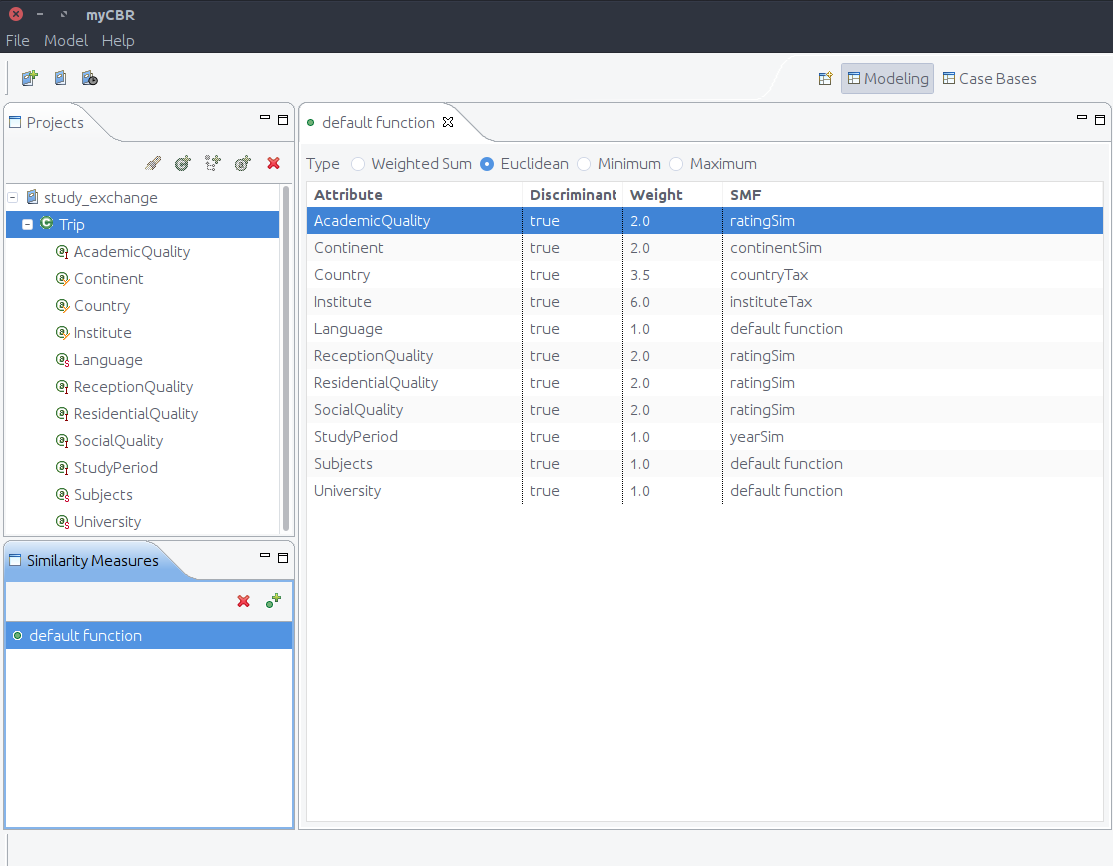
\includegraphics[width=0.8\textwidth]{fig/cbr_model.png}
    \caption{The similarity measure overview in the MyCBR Workbench}
\end{figure}

A Java project was creatd with the MyCBR SDK. This project imports all the parsed cases as a CSV file, and the CBR model created with the MyCBR Workbench. A Java Spring server was implemented to serve the application, with a REST framework to receive requets from Utsida, and serve back a list of the most similar cases to the query. Finally, Maven was used to compile a JAR file which runs the CBRS. 

\begin{figure}[H]
    \label{fig:retrieval_process_diagram}
    \centering
    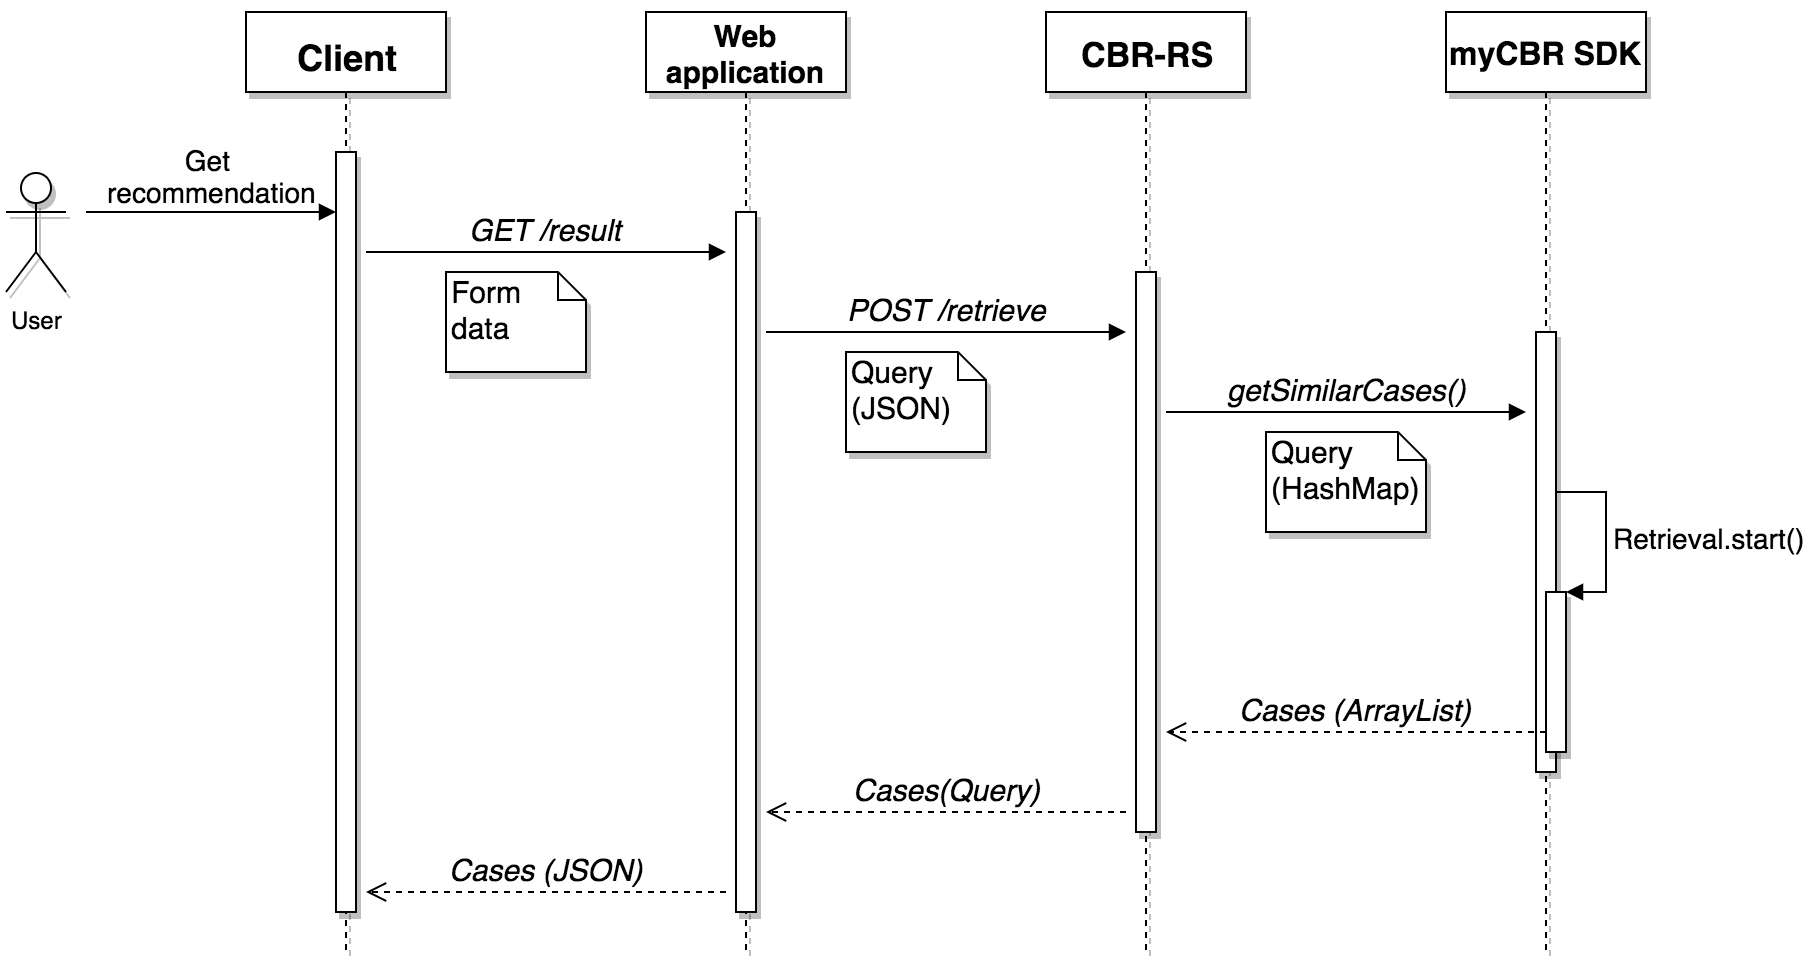
\includegraphics[width=0.8\textwidth]{fig/RetrievalProcessDiagram.png}
    \caption{Sequence diagram which shows how the initial user input is handled before returning as similar cases}
\end{figure}

It is important to note that this process only performs the first step of the CBR-cycle: Retrieval. It returns a set of the most similar cases to a query from Utsida. This makes the system more in line with a Case-Based Recommender System, than a standard CBRS. 

\begin{displayquote}\enquote{
In principle, recommendations need also a query. This query is, however, not asking
for a specific product. It is, rather, in the form of a more general wish. The wish may
not even be formulated explicitly by the customer. If there is a user profile, one may
generate or construct a wish that the customer is likely to have.
The answer or solution to the query problem is an item or a set of items that the
customer may want. This requires knowledge about customer’s preferences.\cite{richter2013case}
}\end{displayquote}

Similar to this definition, the query which the CBR module recieves is a \emph{wish} from a student, containing their most desired attributes, combined with information they have stated in their profile, and it returns not one, but a list of recommendations, so that the user can browse these freely, and produce a choice which may be a combination of several of the recommendations.

\section{Implementation}


\subsection{Components}
This section describes the different components of the system detailed in the previous section. These components build the application that are needed to answer request question 1. They each have a core functionality and use that targets a specific problem domain. 

\paragraph{Reccomendation Handler}
This component of the system handles both the communication with the RESTful MyCBR API as described in the previous part and the views related to the recommendation. The component communicates through http requests and JSON as the data format.

\paragraph{Course Matches}
The main object of the course matches component is to display the approved course matches of a specific university. To enable manually editing and addition by student advisers this components supports add, edit and deletion of course matches. When editing course matches the adviser can add optional comments that include specific information on the course match. The enabled functionality for students include selecting course matches and storing it in the student profile where they can be used in a exchange course application at a later stage. The model fields for course matches include the home course object, abroad course object, approver, approval date, comment and equivalent study points. 

\paragraph{Profile}
This component handles all the user related operation from logging in, changing user data and saving related user data. The data connected to each user profile is institute, saved course matches, saved home courses and saved abroad courses. The stored data is mainly used by the course matcher site, where user can combine a home and abroad course to a custom course match that can further used in an application. 

\paragraph{Applications}
In order to get custom course matches approved a user has to send in an application. This components handles that process and manages application for both the user and the adviser. Allowing users to view, edit and delete an application, while advisers can approve or disapprove an application. 

\subsection{Development process}
The final result data needed in this research requires real users. It was therefore essential that Utsida, which is the surrounding system- and the platform the users actually use, is easy and intuitive to use. To ensure this, the development of Utsida was done in an iterative manner. This included communication with potential users throughout the development, and also usability testing. 

\begin{figure}[h]
    \centering
    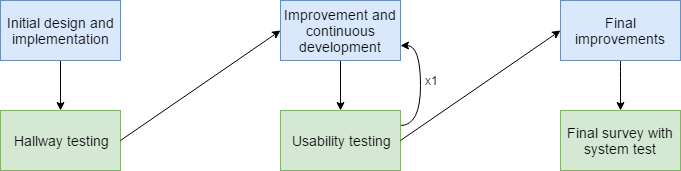
\includegraphics[width=0.9\textwidth]{fig/development_process.png}
    \caption{The development process of Utsida}
    \label{fig:development_process}
\end{figure}

This way, elements which was hard or not very intuitive could be changed before beeing too deep integrated in the system.


\subsection{Design \& Usability}

\subsubsection{Usability Testing}
Each of the two usability test sessions during the development of Utsida produced three System Usability Scale (SUS)-schemas to measure the usability of the system. These were considered in additional to any direct feedback received after each test, as it was ideal to see and increase in these scores during the development. The first session of usability testing yielded the following SUS-scores (1-100): 67.5, 87.5 and 70, while the second session yielded as follows: 92.5, 95 and 97.5. The latter score suggested that the system was in an acceptable state to perform the final survey after the second session of usability testing.

\subsection{Test Environment}
To be able to perform offline usability testing and larger scale online tests the application was hosted on a virtual server provided by Department of Computer Science at NTNU. The virtual server was running Ubuntu 16.04, a debian based linux operating system. The provided domain for the application was utsida.idi.ntnu.no.

The specific HTTP web server used was Apache2, and it was configured with HTTPS to enable secure and encrypted user sessions. To reduce the effort of running online usability tests and enable users to log in through their university account a service platform using UNINETT's federated authentication service (FEIDE) was implemented. The service platform "Dataporten"\cite{dataporten} provided by UNINETT enables quick access to important user data and makes possible application users able to log in without registering a user. 

Error reporting through email was configured on the server so that alerts were given in case of possible downtime or server errors. Error reporting made it possible to quickly resolve potential bugs or errors on the application and ensure higher user satisfaction when running user tests. Tracking user behaviour and statistics could be useful in the final data analysis. Google Analytics was therefore used to increase the understanding of user behaviour. Through Google Analytics it is possible to see a large set of data on the user behaviour. The most important ones used in this project were number of users, average session time, device type and activity flow.  

\cleardoublepage